\documentclass[border=12pt]{standalone}
\usepackage[utf8]{inputenc}
\usepackage[utf8]{vietnam} %Bien dich duoc tieng Viet
\usepackage{amsmath,amsfonts,amssymb} %Font toan
\usepackage{tikz}
\usetikzlibrary{arrows, decorations.markings, calc, fadings, decorations.pathreplacing, patterns, decorations.pathmorphing, positioning}
%\tikzstyle{every path}=[line width=1.2pt]
\newcommand{\drawe}{\draw[line width=1.2pt]}
\newcommand{\bigf}[1]{\Large{#1}} % Ký hiệu cho máy phát
\newcommand{\bbigf}[1]{\huge{#1}} % Tên của các phần tử
\begin{document}
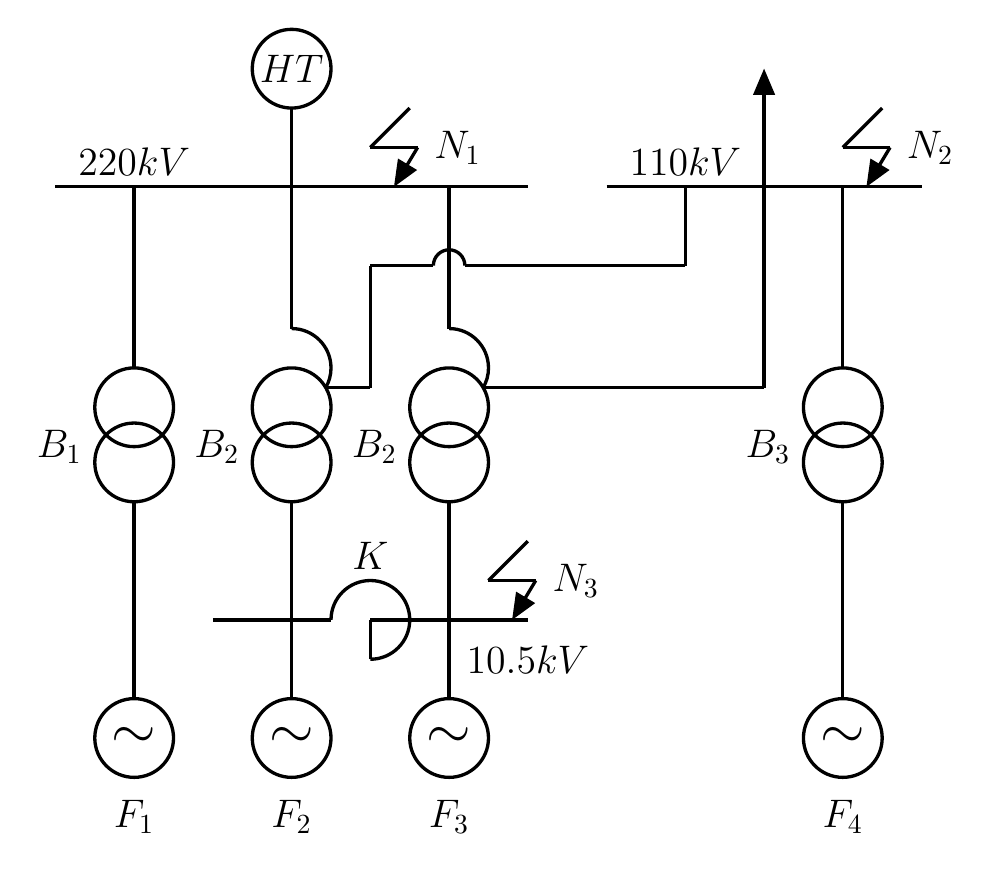
\begin{tikzpicture}[>=triangle 45]
%\draw[color=blue] (-2,-2) grid (11,11); %Tạo lưới

%Nhánh Máy phát F1
\drawe (0,0) circle [radius=0.5] node {\bbigf{$\sim$}};	%Vẽ máy phát
\drawe (0,-1) node {\bigf{$F_1$}};
\drawe (0,0.5) -- (0,3);		%Nối máy phát - máy biến áp
\drawe (0,3.5) circle [radius=.5]; %Vẽ máy biến áp
\drawe (0,4.2) circle [radius=.5];
\drawe (0,3.7) node[left=15pt] {\bigf{$B_1$}};
\drawe (0,4.7) -- (0,7); % Nối máy biến áp với thanh cái

%Nhánh máy phát F2
\drawe (2,0) circle [radius=0.5] node {\bbigf{$\sim$}};	%Vẽ máy phát
\drawe (2,-1) node {\bigf{$F_2$}};
\drawe (2,0.5) -- (2,3);		%Nối máy phát - máy biến áp
\drawe (2,3.5) circle [radius=.5]; %Vẽ máy biến áp
\drawe (2,4.2) circle [radius=.5];
\drawe (2,3.7) node[left=15pt] {\bigf{$B_2$}};
\drawe (2.5,4.7) arc (0:90:.5); 	% Phần máy biến áp tự ngẫu
\drawe (2.5,4.7) arc (0:-30:.5); %
\drawe (2,5.2) -- (2,7);	% Nối máy biến áp với thanh cái
%Nhánh máy phát F3
\drawe (4,0) circle [radius=0.5] node {\bbigf{$\sim$}};	%Vẽ máy phát
\drawe (4,-1) node {\bigf{$F_3$}};
\drawe (4,0.5) -- (4,3);		%Nối máy phát - máy biến áp
\drawe (4,3.5) circle [radius=.5]; %Vẽ máy biến áp
\drawe (4,4.2) circle [radius=.5];
\drawe (4,3.7) node[left=15pt] {\bigf{$B_2$}};
\drawe (4.5,4.7) arc (0:90:.5); 	% Phần máy biến áp tự ngẫu
\drawe (4.5,4.7) arc (0:-30:.5); %
\drawe (4,5.2) -- (4,7);	% Nối máy biến áp với thanh cái

%Nhánh máy phát F4
\drawe (9,0) circle [radius=0.5] node {\bbigf{$\sim$}};	%Vẽ máy phát
\drawe (9,-1) node {\bigf{$F_4$}};
\drawe (9,0.5) -- (9,3);		%Nối máy phát - máy biến áp
\drawe (9,3.5) circle [radius=.5]; %Vẽ máy biến áp
\drawe (9,4.2) circle [radius=.5];
\drawe (9,3.7) node[left=15pt] {\bigf{$B_3$}};
\drawe (9,4.7) -- (9,7);

% Nối các phần tử với nhau
\drawe (-1,7) -- (5,7);
\drawe (6,7) -- (10,7);
\drawe (2,7) -- (2,8); %Nối thanh cái với hệ thống
\drawe (2,8.5) circle [radius=0.5] node {\bigf{$HT$}}; %Vẽ hệ thống
%Nối máy biến áp với thanh cái
\drawe (2.45,4.45) -- (3,4.45); % Nối dây biến áp tự ngẫu B2
\drawe (3,4.45) -- (3,6);
\drawe (3,6) -- (3.8,6);
\drawe (4.2,6) arc (0:180:.2);
\drawe (4.2,6) -- (7,6);
\drawe (7,6) -- (7,7);
\drawe (4.45,4.45) -- (8,4.45); % Nối dây biến áp tự ngẫu B3
\drawe (8,4.45) -- (8,7);

% Vẽ cuộn kháng
\drawe (1,1.5) -- (2.5,1.5);
\drawe (3.5,1.5) arc (0:180:.5);
\drawe (3.5,1.5) arc (0:-90:.5);
\drawe (3,1) -- (3,1.5);
\drawe (3,1.5) -- (3.5,1.5);
\drawe (3.5,1.5) -- (5,1.5);
\drawe (3,2) node[above] {\bigf{$K$}};

%Điện áp thanh cái
\drawe (0,7) node[above] {\bigf{$220kV$}};
\drawe (7,7) node[above] {\bigf{$110kV$}};
\drawe (5,1) node {\bigf{$10.5kV$}};

%Vẽ điểm ngắn mạch
\drawe (3.5,8) -- (3,7.5);	% Tại N1
\drawe (3,7.5) -- (3.6,7.5);
\drawe[->] (3.6,7.5) -- (3.3,7);
\drawe (3.5,7.5) node[right=5pt] {\bigf{$N_1$}};
\drawe (9.5,8) -- (9,7.5);	% Tại N2
\drawe (9,7.5) -- (9.6,7.5);
\drawe[->] (9.6,7.5) -- (9.3,7);
\drawe (9.5,7.5) node[right=5pt] {\bigf{$N_2$}};
\drawe[->] (8,7) -- (8,8.5); %Vẽ phụ tải tại 110kV
\drawe (5,2.5) -- (4.5,2);	% Tại N3
\drawe (4.5,2) -- (5.1,2);
\drawe[->] (5.1,2) -- (4.8,1.5);
\drawe (5,2) node[right=5pt] {\bigf{$N_3$}};
\end{tikzpicture}
\end{document}